\documentclass[mathserif]{beamer}
\usepackage[ngerman]{babel}
\usepackage[latin1]{inputenc}
\usepackage{amsmath, amssymb}
\usepackage{latexsym}
%
\newcommand{\R}{\mathbb{R}}
\usetheme{Madrid}
\usecolortheme{seahorse}
%
%
\title[MNS Project 2]{MNS Project 2: Learning of Grid Cells}
\author[C. Lang, E. Sezener, C.Winklmayr]{Claus Lang, Eren Sezener and Claudia Winklmayr}
\institute{BCCN}
\date[9.2.2016]{February $9^{th}$ 2016}
%
\begin{document}
\maketitle
%
%
%
\begin{frame}
\frametitle{Structure}
	\begin{itemize}
	\item Introduction\newline
	\item Modelling details\newline
	\item Results
	\end{itemize}
\end{frame}
%
%
%
\begin{frame}
\frametitle{Introduction}
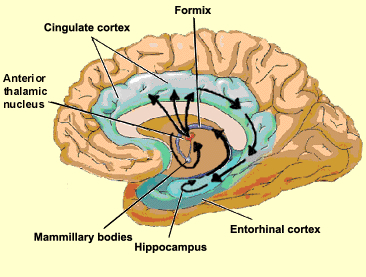
\includegraphics[width=0.7\textwidth]{mEC.jpg}\newline
%http://www.irafs.org/images/irafs_nl_eng_2_files/image007.jpg
In Hippocampus and the medial enthorhinal cortex (mEC) various types of neurones have been found that encode an animals spacial location.  
\end{frame}
% 
%
%
\begin{frame}
\frametitle{Cells encoding spacial location}
\begin{itemize}
\item \textbf{Place cells} \newline
%Located in hippocampus. Activated when the animal enters a specific region of the environment - the \textit{place field]}. \newline
%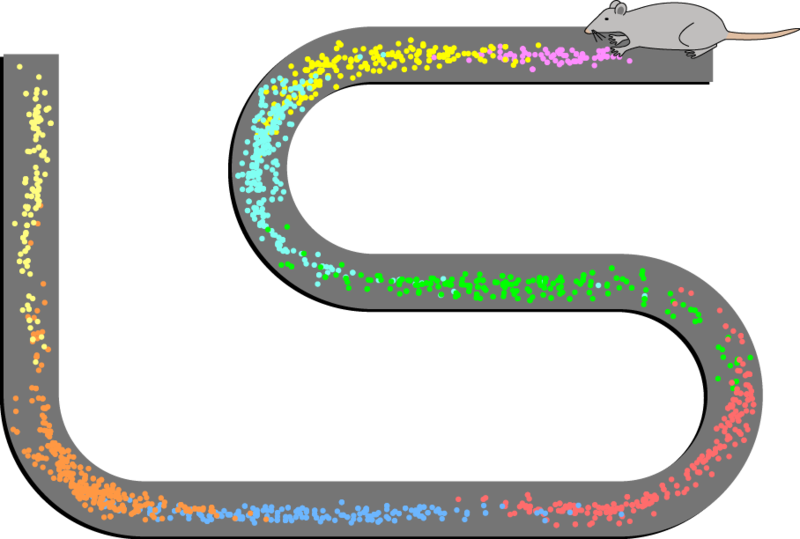
\includegraphics[width=0.33\textwidth]{Place_Cell_Spiking_Activity_Example.png}
%"Place Cell Spiking Activity Example" by Stuartlayton at English Wikipedia. Licensed under CC BY-SA 3.0 via Commons - https://commons.wikimedia.org/wiki/File:Place_Cell_Spiking_Activity_Example.png#/media/File:Place_Cell_Spiking_Activity_Example.png
\item \textbf{Grid cells} \newline
%Located in  medial enthorhinal cortex (mEC). Activated at several spacial positions. The firing map shows an equally spaced hexagonal pattern. \newline
\item \textbf{Head-direction cells}\newline
\item \textbf{Head-Grid-Conjunctive cells}
\end{itemize}
\end{frame}
%
%
%
\begin{frame}
\frametitle{Properties of place cells}
\begin{columns}[T]
    \begin{column}{.5\textwidth}
			Located in hippocampus. Activated when the animal enters a specific region of the environment - the \textit{place field}.
    \end{column}
    \begin{column}{.5\textwidth}
    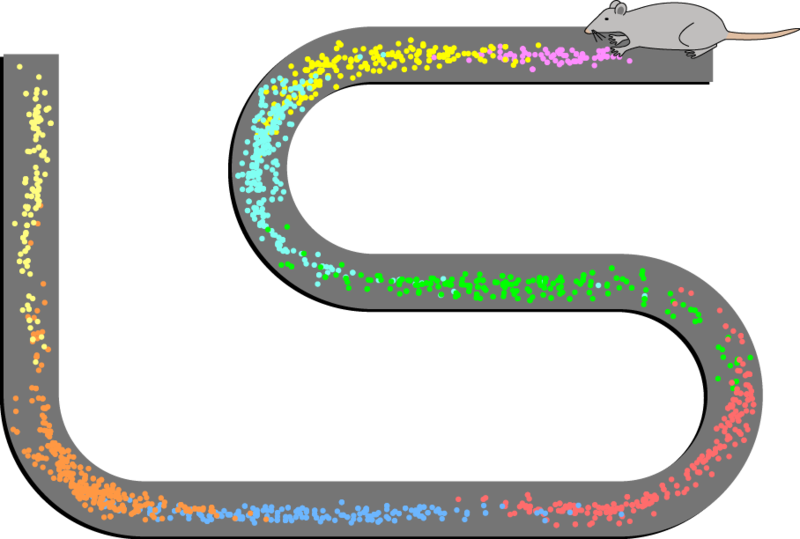
\includegraphics[width=0.9\textwidth]{Place_Cell_Spiking_Activity_Example.png}
    \end{column}
  \end{columns}	
\end{frame}
%
%
%
\begin{frame}
\frametitle{Properties of grid cells}
\begin{columns}[T]
    \begin{column}{.5\textwidth}
			\begin{itemize}
			\item Located in  medial enthorhinal cortex (mEC). Activated at several spacial positions. The firing map shows an equally spaced hexagonal pattern. 
			%\item Perform path integration i.e. process information about location, direction, speed
			\item Mostly independent of visual stimulus
			\item Different grid cells show diffrend spacing, orientation and size of their patterns.
			\item Spacing from 25cm to 3m. 
			\end{itemize}
    \end{column}
    \begin{column}{.5\textwidth}
    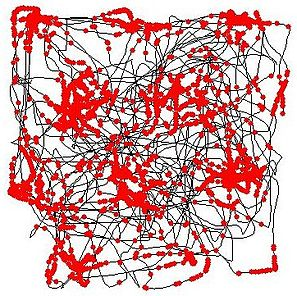
\includegraphics[width= 0.9\textwidth]{RatRunningPath.JPG}
    \end{column}
  \end{columns}	
\end{frame}
%
%
%
\begin{frame}
\frametitle{Rat trajectory}
  \begin{columns}[T]
    \begin{column}{.5\textwidth}
			\begin{itemize}
		    \item Square environment of size $125 \times 125$ cm.
		    \item Speed: $v=0.4$ m/s
		    \item Initialization with random position
		    \item Every 10ms: chose new direction from a gaussian distibution with 
		    	\begin{itemize}
		    	\item $\mu=$ previous direction
		    	\item $\sigma= 0.2$
		    	\end{itemize}
		    \end{itemize}
    \end{column}
    \begin{column}{.5\textwidth}
    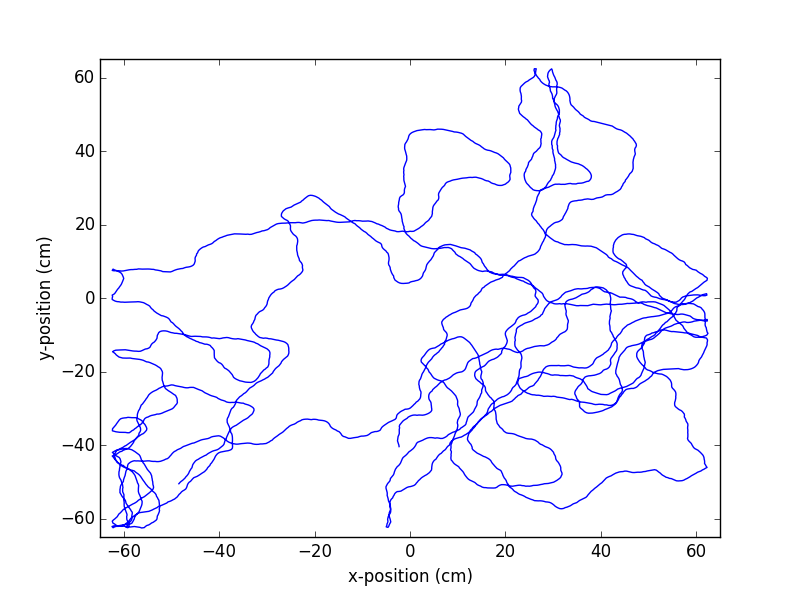
\includegraphics[width=6cm]{running_rat.jpeg}
    %\caption{running time: 5 seconds}
    \end{column}
  \end{columns}
\end{frame}


\end{document}
%